\documentclass[hyperref=unicode]{beamer}

\usepackage[absolute,overlay]{textpos}
\usepackage{graphicx}
\usepackage{adjustbox}
\usepackage{mhchem}
\usepackage{wrapfig}
\usepackage{ucs}
\usepackage[utf8]{inputenc}
\PrerenderUnicode{ěščřžýáíéĚŠČŘŽÝÁÍÉďťňĎŤŇůúÚóÓ}

\usepackage{multirow}

\adjustboxset*{center}

\mode<presentation>{\usetheme{Madrid}}
\DefineNamedColor{named}{pozadi}{RGB}{200,200,200}
\usecolortheme{crane}

\setbeamertemplate{footline}[frame number]
\usepackage[czech]{babel}
\usepackage[T1]{fontenc}
\usepackage{lmodern}

\addtobeamertemplate{frametitle}{
   \let\insertframetitle\insertsectionhead}{}
\addtobeamertemplate{frametitle}{
   \let\insertframesubtitle\insertsubsectionhead}{}

\makeatletter
  \CheckCommand*\beamer@checkframetitle{\@ifnextchar\bgroup\beamer@inlineframetitle{}}
  \renewcommand*\beamer@checkframetitle{\global\let\beamer@frametitle\relax\@ifnextchar\bgroup\beamer@inlineframetitle{}}
\makeatother
\setbeamercolor{section in toc}{fg=blue}
\setbeamertemplate{section in toc shaded}[default][100]

\usepackage{tikz}
\usetikzlibrary{positioning}
\usetikzlibrary{arrows}
\usetikzlibrary{shapes.multipart}

\begin{document}

\title[Crisis]{Chemická kinetika}

\subtitle{Rovnováhy, rychlost chemických reakcí}

%Reakční kvocient, Guldberg-Waagův zákon, Le-Chatelierův princip, závislost reakční konstanty na teplotě, tlaku a koncentraci, rychlost a řád reakce, rozsah chemické reakce

\author{Zdeněk Moravec, hugo@chemi.muni.cz \\ 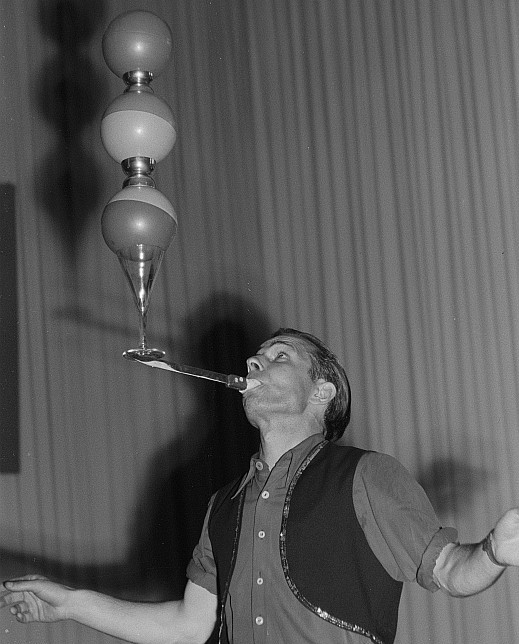
\includegraphics[keepaspectratio,width=4cm]{balance.jpg}}

\frame{\titlepage}

\section{Chemická kinetika}
\frame{
	\frametitle{}
	\vfill
	\begin{itemize}
	\item Rychlost chemických reakcí
	\begin{itemize}
	\item Závislost koncentrace na čase
	\item Rychlost je ovlivněna počáteční koncentrací reaktantů, teplotou, přítomností katalyzátoru, \ldots
	\end{itemize}
	\item Reakční mechanismus
	\end{itemize}
	\vfill
}

\section{Rovnováha chemické reakce}
\subsection{1. Faradayův zákon}
\frame{
	\frametitle{}
	\vfill
	\begin{itemize}
	\item Probíhá v roztocích nebo taveninách
	\item Elektrolýze může podléhat rozpouštědlo nebo ionty elektrolytu
	\item \ce{2 H2O -> 2 H2 + O2}
	\item \textbf{1. Faradayův zákon}
	\item Hmotnost vyloučené látky je úměrná proudu, který prochází elektrolytem a času, po který elektrolýza probíhala
	\item $m = A.I.t = A.Q$
	\begin{itemize}
	\item A - elektrochemický ekvivalent, I - proud, t - čas, Q - náboj
	\end{itemize}
	\end{itemize}
	\vfill
}

\end{document}